% Generated by paper/figures/src/fig_phase2.py 6144; do not edit by hand.
% Generated by fig_phase2.py 6144; frozen selection in gallery_6144/provenance.json.
% 880657115260655727: A stone bridge with arched spans reflects golden light on the water, flanked by buildings and a leafy tree under a clear blue sky.
% m2014927182109364975: A panoramic view of Paris featuring the Eiffel Tower, the Seine River, and various ornate buildings with greenery and bustling activity, including boats on the water and crowds along walkways.
% m4012780704267384036: A woman in a white dress with cape sleeves stands on a rooftop holding a black clutch, against a blurred city skyline and overcast sky.
% m5685677173773420545: A muscular, bald man holds a flower above his head with both arms, set against a soft circular background in black and white.
\begin{figure*}[t]
\centering\sffamily\scriptsize\ifdefined\scaW\else\newlength{\scaW}\fi\setlength{\scaW}{\textwidth}
\setlength{\fboxsep}{1pt}\setlength{\lineskip}{0pt}\setlength{\lineskiplimit}{0pt}
\makebox[\textwidth][l]{\makebox[0.4975\scaW][c]{AReA}\hspace{0.0040\scaW}\makebox[0.4975\scaW][c]{\textbf{SCA (ours)}}}\\[0.0040\textwidth]
\makebox[\textwidth][l]{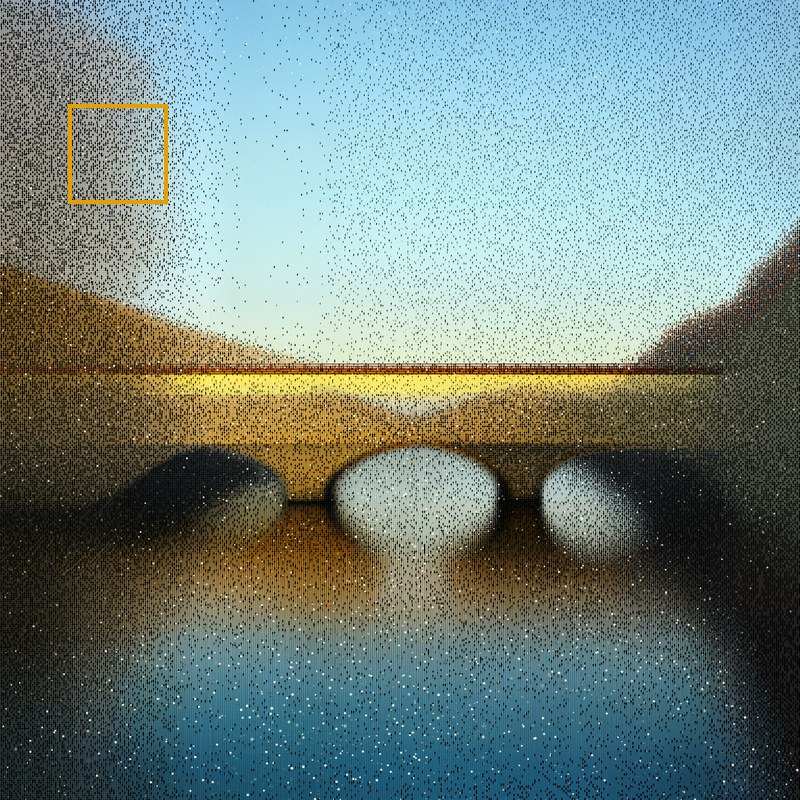
\includegraphics[height=0.2467\scaW]{figures/gallery_6144/880657115260655727_area.jpg}\hspace{0.0040\scaW}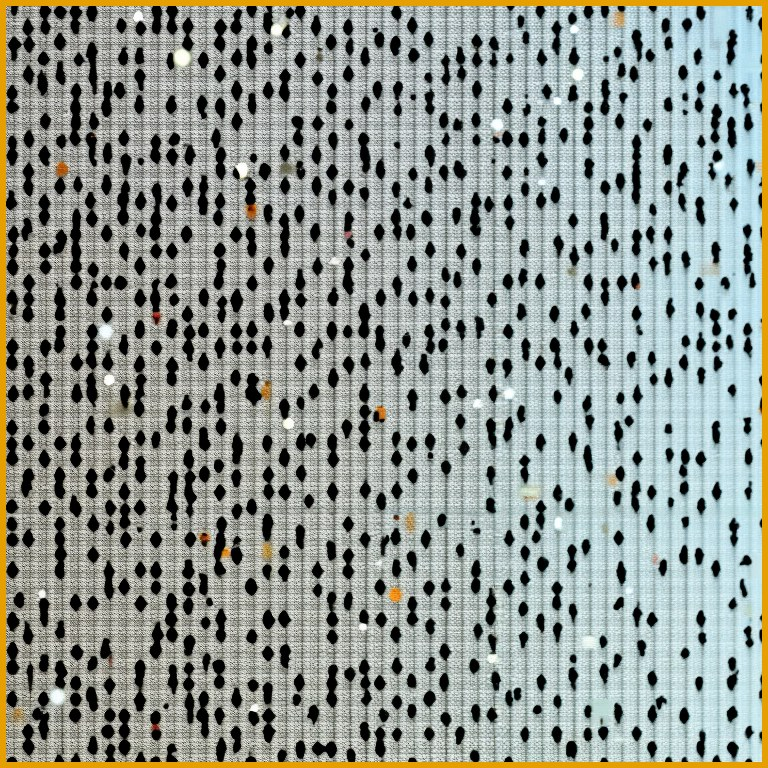
\includegraphics[height=0.2467\scaW]{figures/gallery_6144/880657115260655727_area_crop.jpg}\hspace{0.0040\scaW}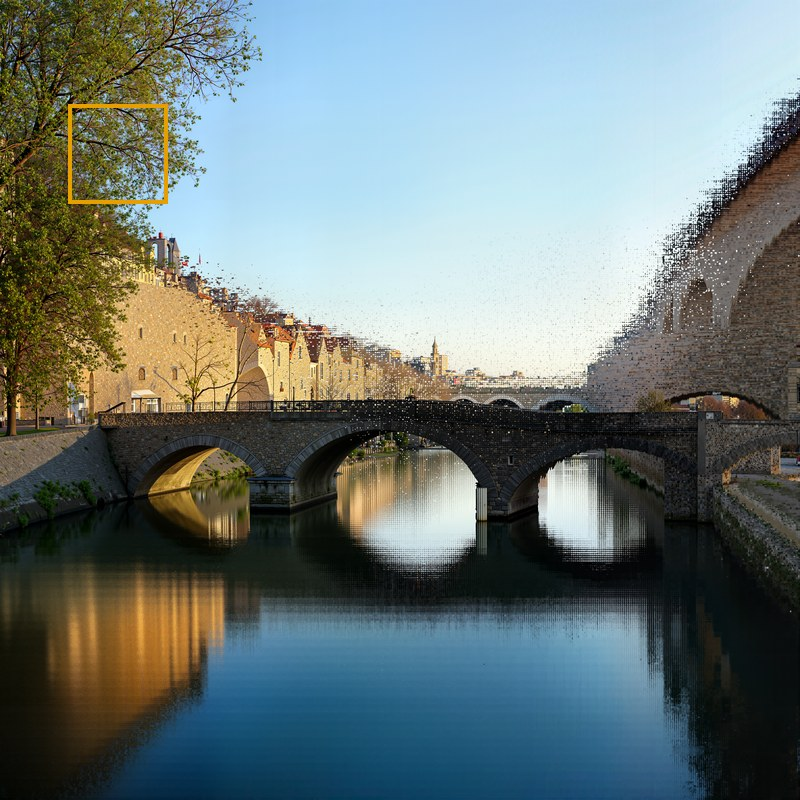
\includegraphics[height=0.2467\scaW]{figures/gallery_6144/880657115260655727_sca.jpg}\hspace{0.0040\scaW}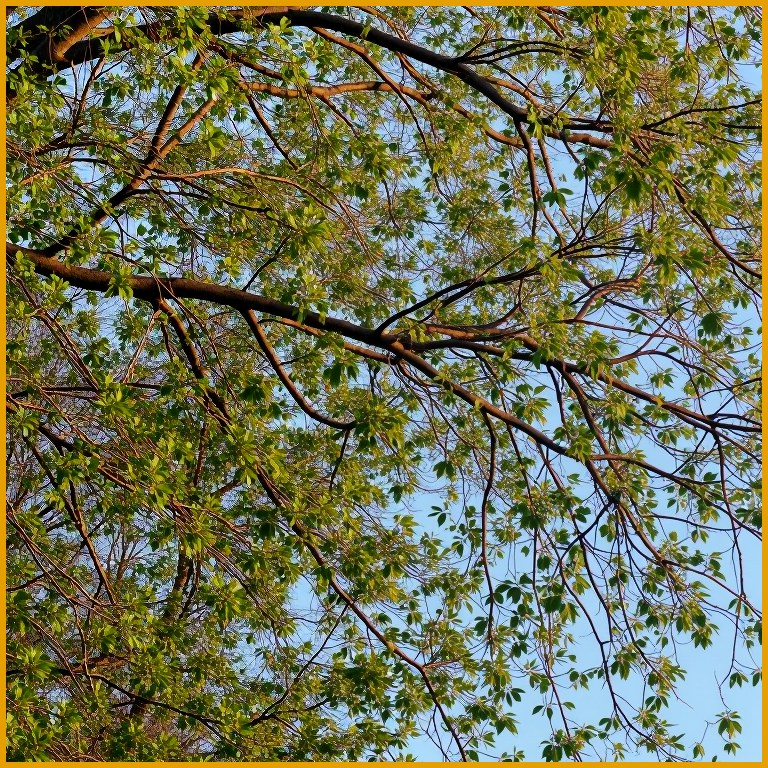
\includegraphics[height=0.2467\scaW]{figures/gallery_6144/880657115260655727_sca_crop.jpg}}\\[0.0040\textwidth]
\makebox[\textwidth][l]{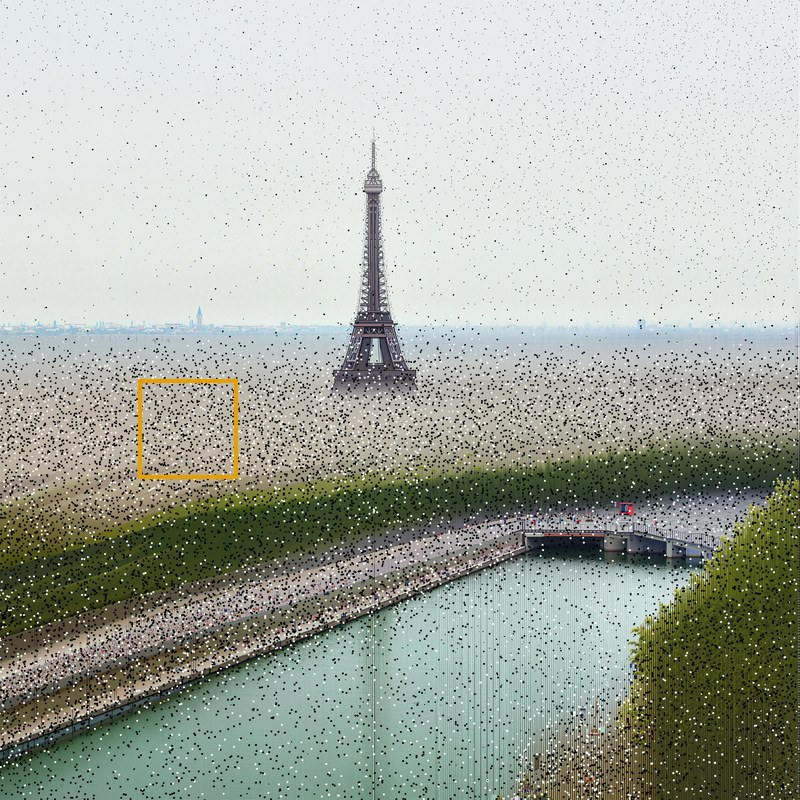
\includegraphics[height=0.2467\scaW]{figures/gallery_6144/m2014927182109364975_area.jpg}\hspace{0.0040\scaW}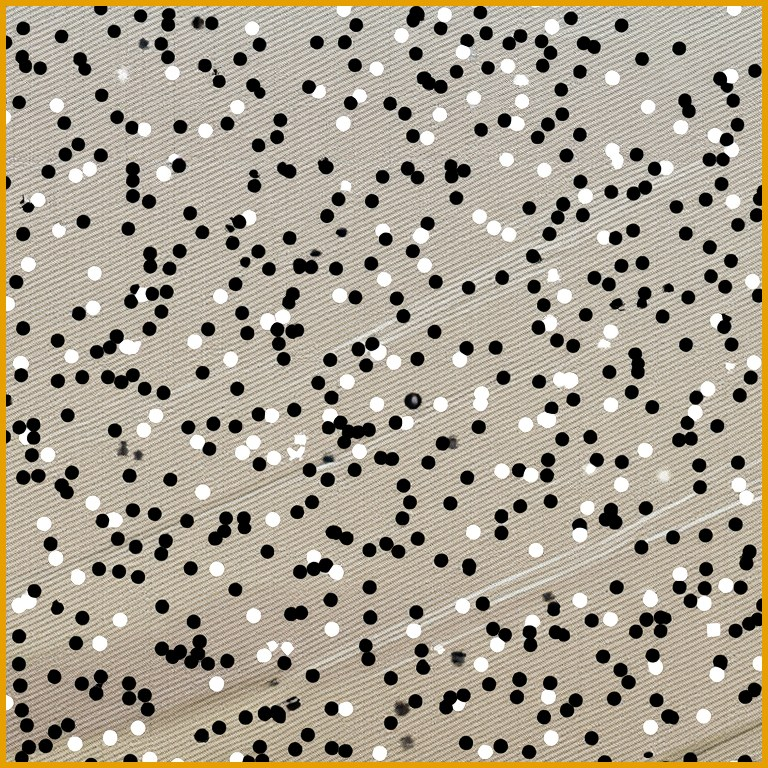
\includegraphics[height=0.2467\scaW]{figures/gallery_6144/m2014927182109364975_area_crop.jpg}\hspace{0.0040\scaW}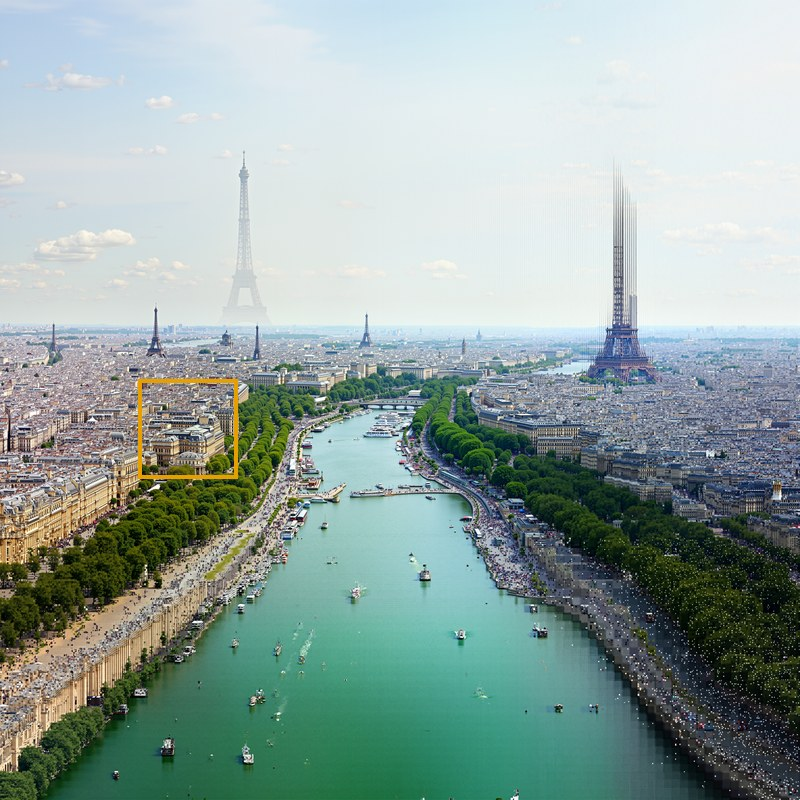
\includegraphics[height=0.2467\scaW]{figures/gallery_6144/m2014927182109364975_sca.jpg}\hspace{0.0040\scaW}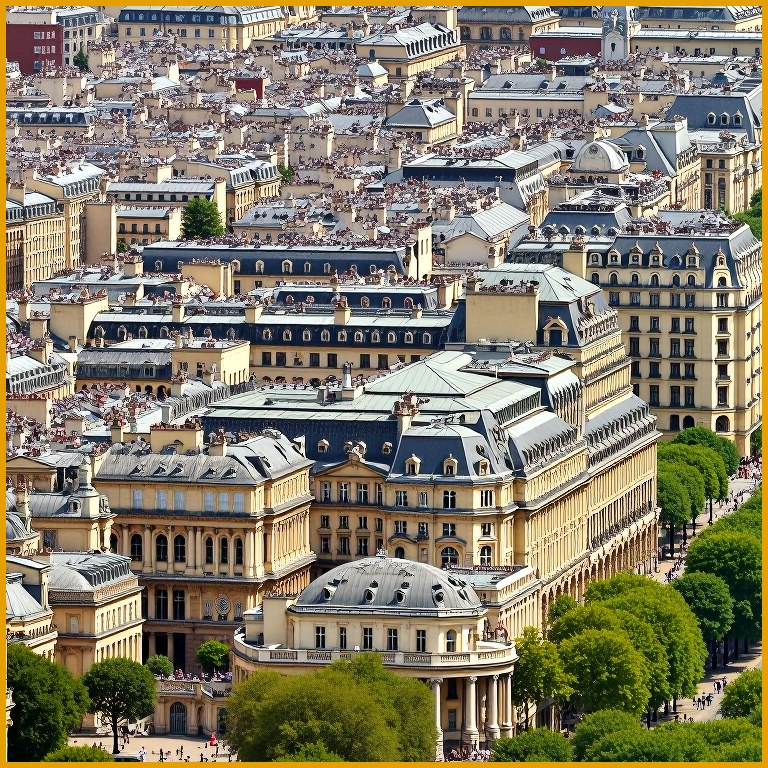
\includegraphics[height=0.2467\scaW]{figures/gallery_6144/m2014927182109364975_sca_crop.jpg}}\\[0.0040\textwidth]
\makebox[\textwidth][l]{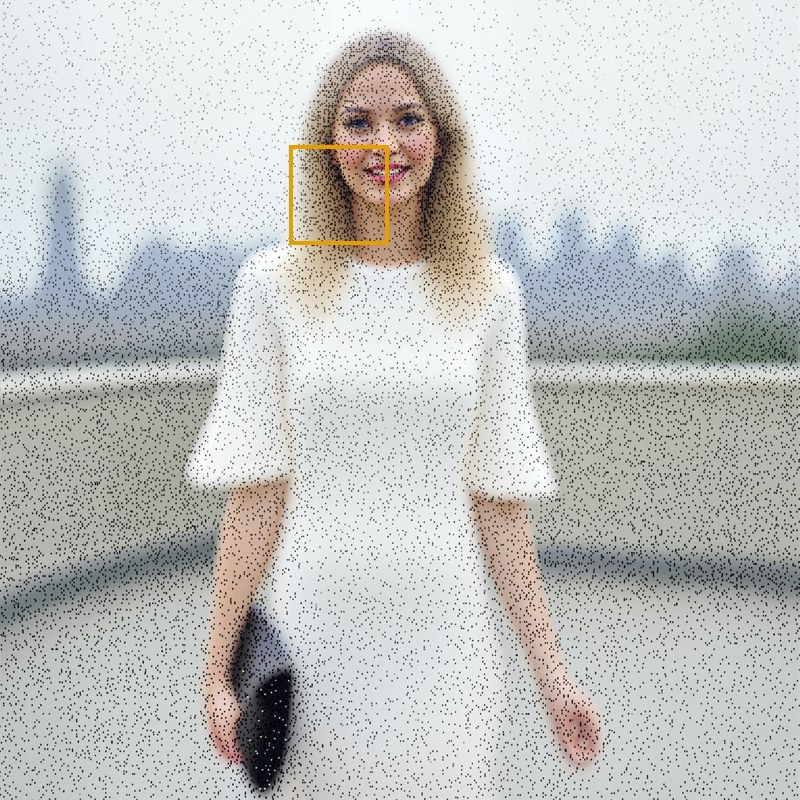
\includegraphics[height=0.2467\scaW]{figures/gallery_6144/m4012780704267384036_area.jpg}\hspace{0.0040\scaW}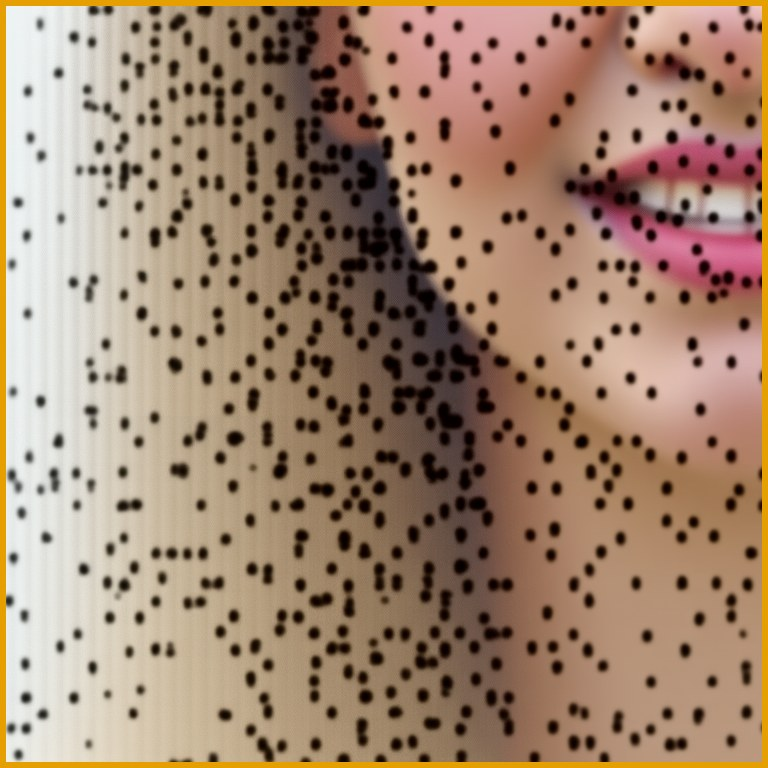
\includegraphics[height=0.2467\scaW]{figures/gallery_6144/m4012780704267384036_area_crop.jpg}\hspace{0.0040\scaW}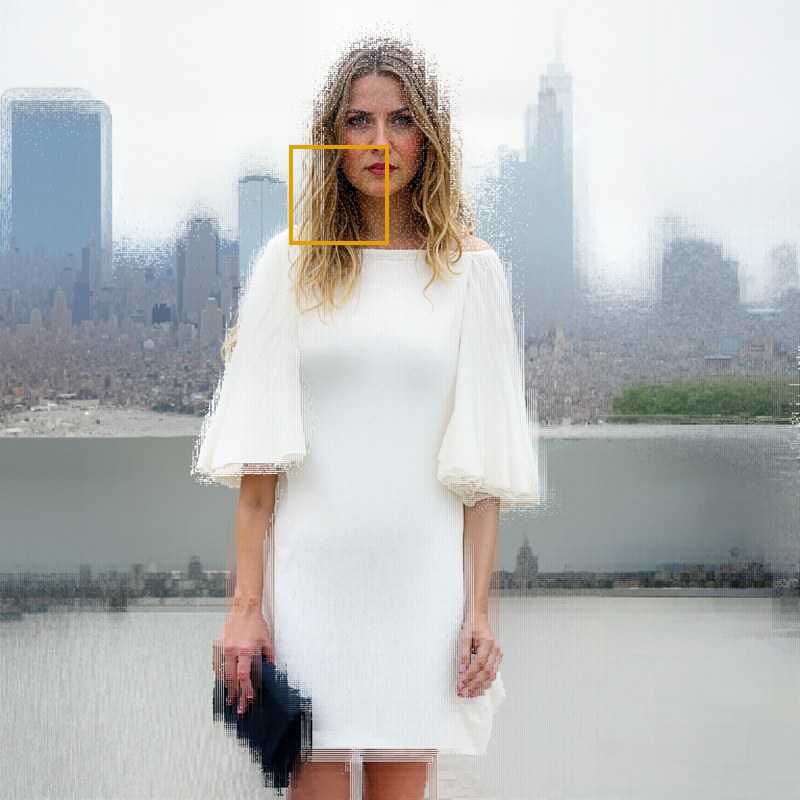
\includegraphics[height=0.2467\scaW]{figures/gallery_6144/m4012780704267384036_sca.jpg}\hspace{0.0040\scaW}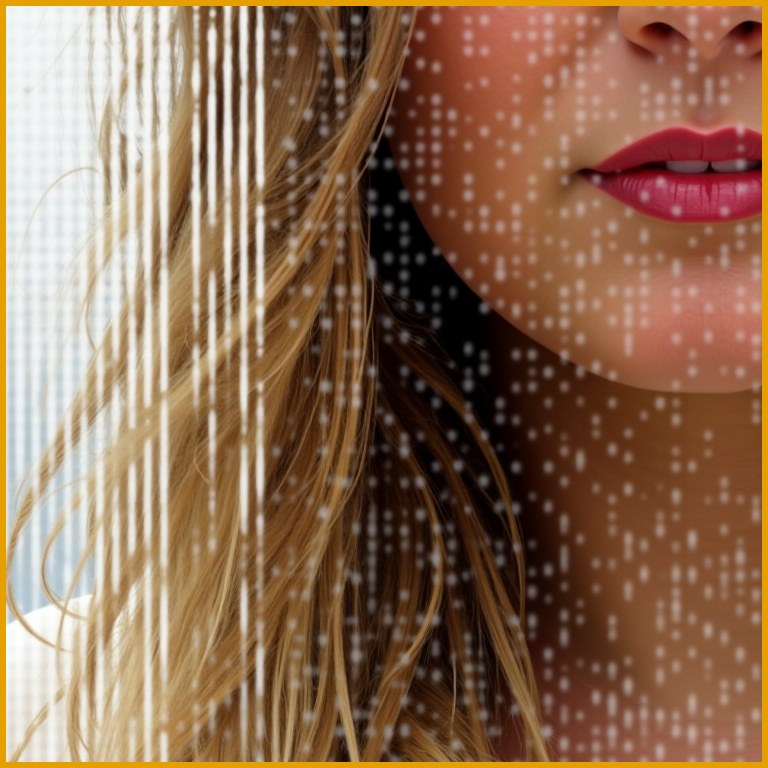
\includegraphics[height=0.2467\scaW]{figures/gallery_6144/m4012780704267384036_sca_crop.jpg}}\\[0.0040\textwidth]
\makebox[\textwidth][l]{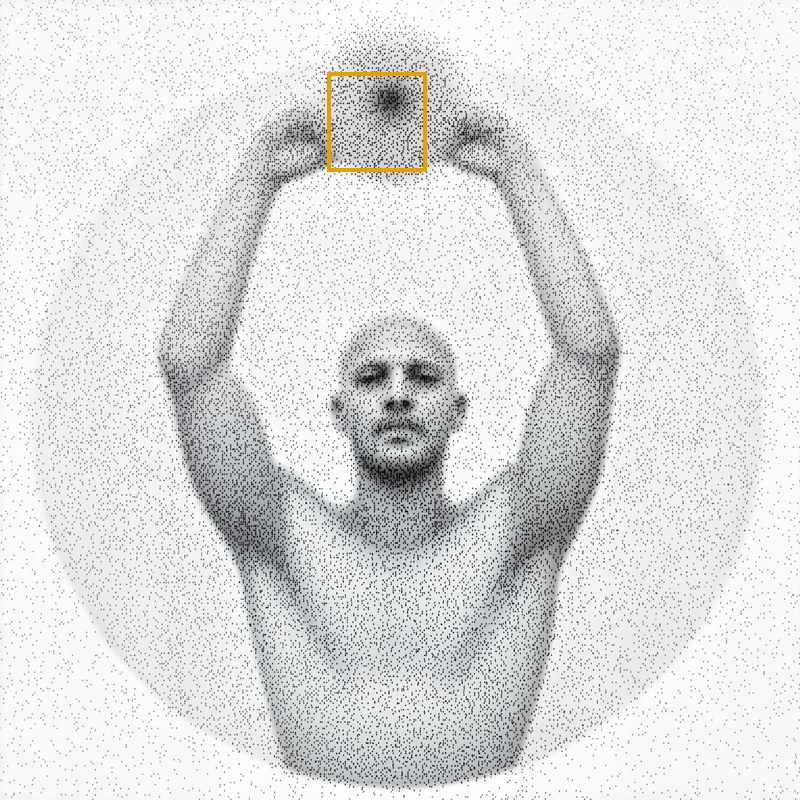
\includegraphics[height=0.2467\scaW]{figures/gallery_6144/m5685677173773420545_area.jpg}\hspace{0.0040\scaW}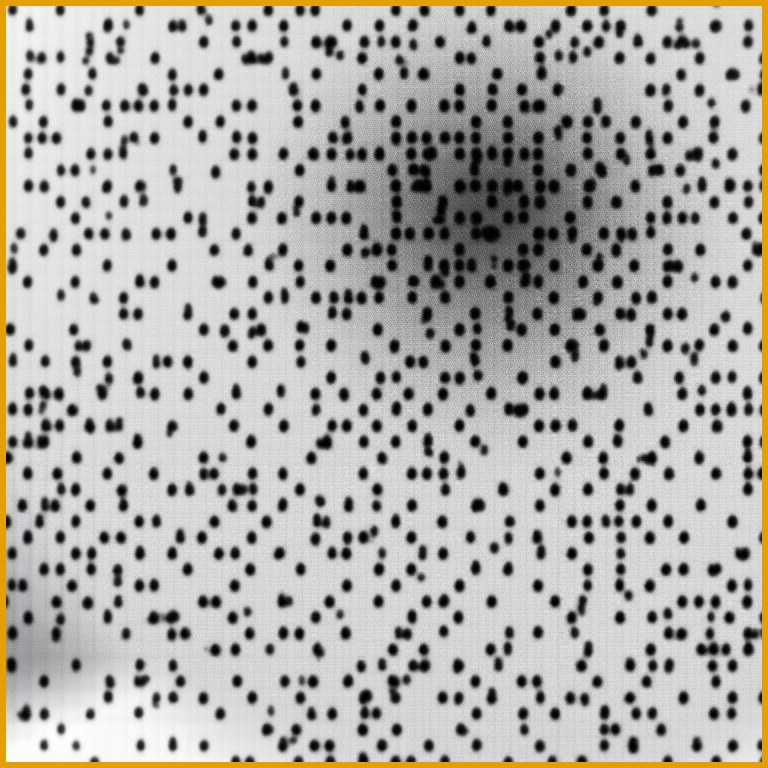
\includegraphics[height=0.2467\scaW]{figures/gallery_6144/m5685677173773420545_area_crop.jpg}\hspace{0.0040\scaW}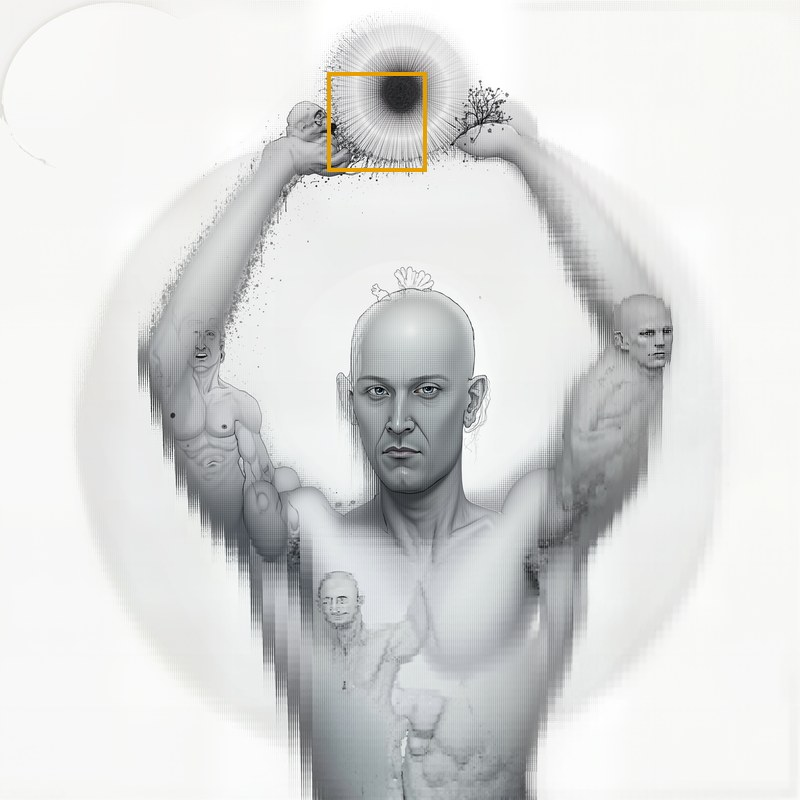
\includegraphics[height=0.2467\scaW]{figures/gallery_6144/m5685677173773420545_sca.jpg}\hspace{0.0040\scaW}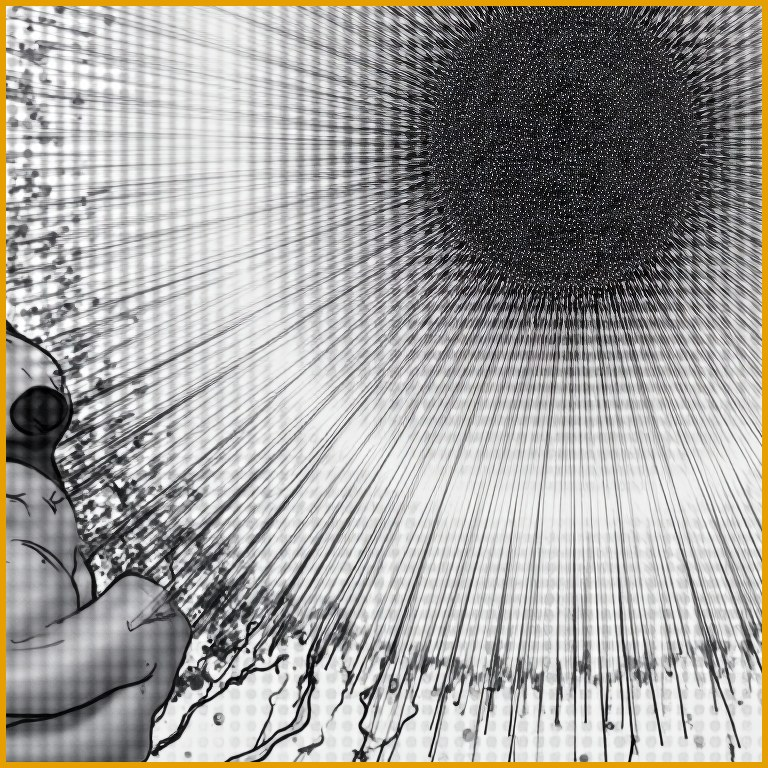
\includegraphics[height=0.2467\scaW]{figures/gallery_6144/m5685677173773420545_sca_crop.jpg}}
\rmfamily\normalsize
\caption{\textbf{Partial qualitative results at $6144^2$.} 4 prompts sampled uniformly from the 14 non-development prompts with completed AReA and SCA outputs at the figure snapshot; this is not the final evaluation set. Each full image is followed by its native-pixel crop. FLUX.1-dev, seed 0, 28 steps, guidance 4.5. The subset was not selected by image quality; completion order may differ from the full benchmark. Crop locations maximize edge energy averaged across the methods shown. Prompt selection uses seed 17; source hashes and crop coordinates are archived with the figure.}
\label{fig:gallery_6144}
\end{figure*}
